\svnid{$Id: plotting_options.tex 80815 2026-02-17 17:10:15Z jagers $}

\chapter{Plotting options} \label{Chp:PlottingOptions}
As already indicated in the `Getting started' chapter, the plot options available in the right part of the window are constantly adjusting to the selections that you make in the left part of the window (different data fields from the data file, different selections of space and time co-ordinates).
Note that the list of options, which is by default docked into the right part of the main window, can also be undocked to a separate window using the undock/dock button at the top right corner of the option list, just above the scroll bar.

\begin{figure}[H]
\center{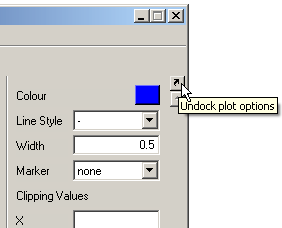
\includegraphics[width=0.48\textwidth]{Ch03/undock.png}
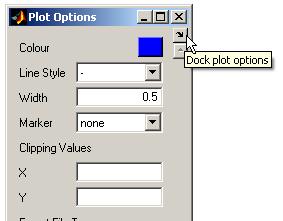
\includegraphics[width=0.48\textwidth]{Ch03/dock.png}}
\caption{Undocking and docking of the plot options.}
\label{fig:3.1}
\end{figure}

This chapter describes all available options.
We will use a 2D vector field (for instance the depth averaged velocity) as the main example since most options apply to it.
Initially the list of options will look as shown in \Fref{fig:3.2}a: the plot will result in a field of blue automatically scaled vectors.

\begin{Remark}
\item The export option is discussed in Chapter 5.
\item Changing an option will only affect the options below it.
The best way to work through the list is from top to bottom.
\item The options interface has been programmed to be ``lazy'', that is, the options retain their setting when switching between data files and data fields.
This helps to make consistent plots of different datasets.
\item If there are more options available than fit on the screen, the slider just to the right of the list of options becomes active and it allows you to scroll through all relevant options (as shown in \Fref{fig:3.2}b).
\end{Remark}

\begin{figure}
\center{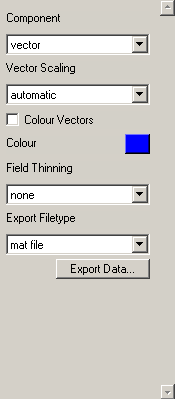
\includegraphics{Ch03/3-1a.png}
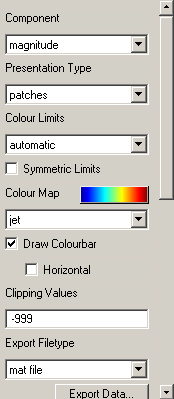
\includegraphics{Ch03/3-1b.png}}
\caption{List of plot options depending on the plot type: (a, left) vector and (b, right) scalar.}
\label{fig:3.2}
\end{figure}

\section{Axes type}
Some data sets may be plotted in different ways.
The axes type selection option allows you the select the type of axes you want to plot the data in.
For a time-dependent dataset the options include 'Time' which can be used to create a moving time line in a time graph, or a clock (see \Autoref{Sec:PlotManager} for more details).

\begin{figure}
\center{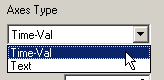
\includegraphics{Ch03/axestype.png}}
\caption{Selecting axes type.}
\label{fig:3.5}
\end{figure}

\section{Time zone}
This option depends on the time zone setting selected in the Preferences dialog, see \Autoref{Sec:Preferences}.
By default the option "Ignore" is selected there, and all time zone information is ignored, and hence no time zone selection option will be shown for the plot.
If you select there "Enforced" then \QUICKPLOT will always use the time zone selected and hence no time zone selection option will be shown for the plot.
Only if you select there "As in Dataset" then \QUICKPLOT will allow you to select the time zone that you want to use in the plot.
However, this option is only available if the plot includes a time axis and the data specifies the time zone.

\section{Plot coordinate}
In the case of a variable defined along a line (or a data slice out of a 3D data set along such a line) you may select any of four coordinates: path distance (distance measured along the line plotted on the horizontal axis), reverse path distance (same as previous option, but measured from the other end), $x$ coordinate and $y$ coordinate.

\begin{figure}[H]
\center{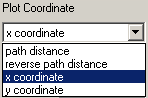
\includegraphics{Ch03/plot_coordinate.png}}
\caption{Selecting plot coordinate.}
\label{fig:3.6}
\end{figure}

\section{Component}
This option is only available for vector quantities.
Basically, it allows you to select between different types of derived quantities.
A vector quantity may be plotted as a vector, but you can also plot its magnitude, direction (according to nautical definition) or one of its components in computational space (M, N) or physical space (X, Y, Z, in plotting plane or perpendicular).
These derived quantities are all scalar quantities, which results in the adjustment of the options below as shown in \Fref{fig:3.2}b.
Plotting a scalar quantity, such as the water level, gives the same options as the plotting of a derived quantity such as the velocity magnitude.

\begin{longtable}{|p{3.5cm}|p{\textwidth-3.5cm-24pt}|}
\caption{Overview of vector components} \\
\hline \STRUT
\textbf{Component} & \textbf{Description} \\ [1ex] \hline \nopagebreak \endhead
\hline
\multicolumn{2}{r}{{\STRUT \tablename\ \thetable{} -- continued on next page}} \\
\endfoot
\endlastfoot
\STRUT vector & vector \\
vector (split $x,y$) & vector plot showing decomposition of vector quantity in $x$ and $y$ components \\
vector (split $m,n$) & vector plot showing decomposition of vector quantity in components in $m$ and $n$ direction \\
magnitude & magnitude of the vector quantity: $(u_x^2+u_y^2+u_z^2)^{1/2}$ \\
magnitude in plane & magnitude of the vector quantity in the selected plane: $(u_m^2+u_z^2)^{1/2}$ in case of a vertical plane along an m grid line \\
normal component & vector component perpendicular to plane: equals n component in case of a vertical plane along an m grid line \\
angle (...) & angle of vector in horizontal plane in degrees or radians clockwise from North (nautical convention) \\
x component & vector component in $x$ direction \\
y component & vector component in $y$ direction \\
z component & vector component in $z$ direction (corresponds to $k$ direction) \\
m component & vector component in local direction of $m$ grid line \\
n component & vector component in local direction of $n$ grid line \\ \hline
\end{longtable}

\begin{figure}[H]
\center{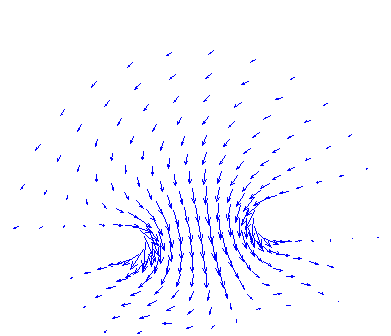
\includegraphics[width=0.5\textwidth]{Ch03/standard_vector_plot.png}}
\caption{Standard vector plot.}
\label{fig:3.4}
\end{figure}

\section{Presentation type}
Depending on the storage of the data field in the data file, there may be several presentation types for 2D plots, such as patches, continuous shades, markers, values, contour lines and contour patches.
Examples are shown in \Fref{fig:3.12}.
The default setting (if available) is patches.

\begin{figure}[H]
\hfill
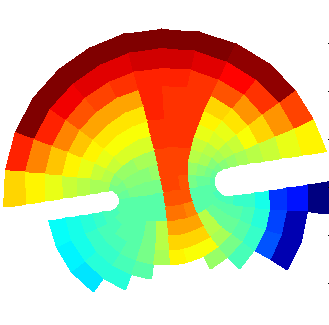
\includegraphics[width=0.3\textwidth]{Ch03/presentation_patches.png}
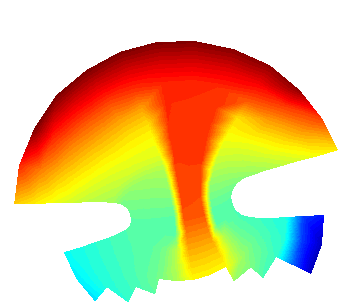
\includegraphics[width=0.3\textwidth]{Ch03/presentation_continuous_shades.png}
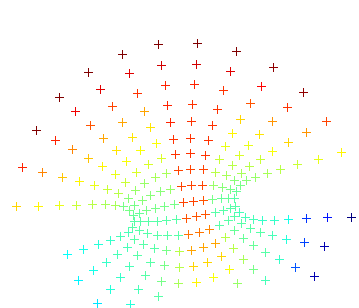
\includegraphics[width=0.3\textwidth]{Ch03/presentation_markers.png}

\hfill
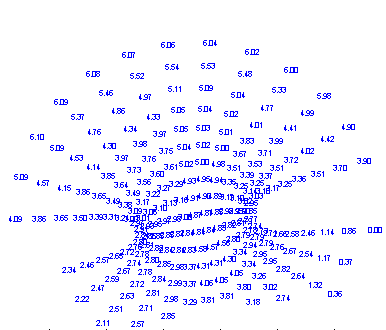
\includegraphics[width=0.3\textwidth]{Ch03/presentation_numbers.png}
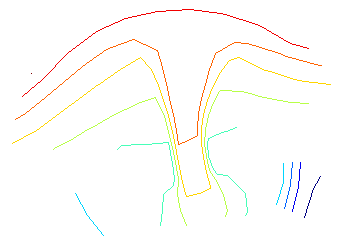
\includegraphics[width=0.3\textwidth]{Ch03/presentation_isolines.png}
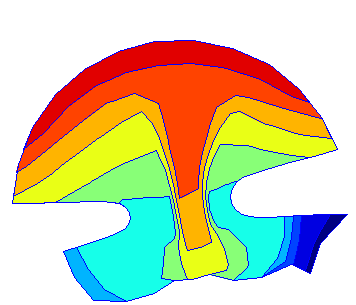
\includegraphics[width=0.3\textwidth]{Ch03/presentation_patches_with_lines.png}

\caption{Examples of the presentation types.}
\label{fig:3.12}
\end{figure}

\begin{Remark}
\item In the case of a patches plot, the uniformly coloured grid cells have their corner points at depth points of the staggered Delft3D grid.
This implies that variables not defined at the water level point (such as the bed levels in their traditional location) have to be transformed in some way.
The bed level data in the \DFLOW\ map file and the Delft3D communication file are processed in accordance with the selected drying-flooding criterion.
Other variables and bed levels stored in files without information on the drying-flooding procedure are averaged to the water level points.
\item In the case of a continuous shades plot or a contour (lines or patches) plot data is linearly interpolated between the points at which the values are defined.
The interpolation is carried out across any thin dams that may exist.
Furthermore, if the values are defined at the water level points in the centre of the grid cells, there will be half of a grid cell missing along the outer rim of the plot area.
Since version 2.15, the option `Extend to Domain Edge' is available to fill in these gaps along the boundaries (see \Fref{fig:extend2edge}).
\item The continuous shades plot is not a 2D plot, but basically a 3D plot.
The values (or when available z-data) is used to generate a 3D surface.
Combining continuous shades plots with other plot types is therefore generally not possible.
\end{Remark}

\begin{figure}[H]
\center{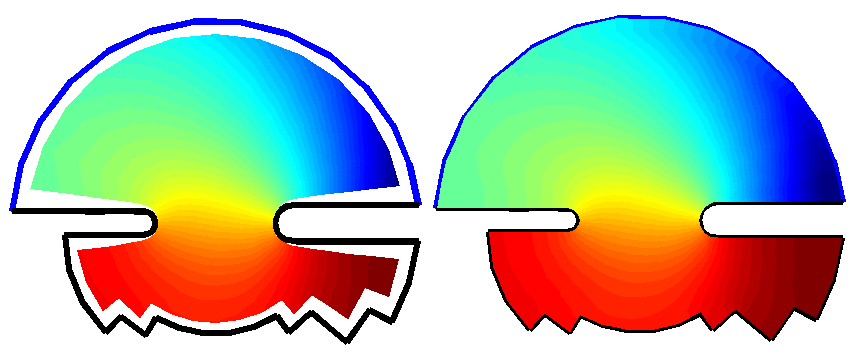
\includegraphics[width=0.7\textwidth]{Ch03/extend2edge.png}}
\caption{Effect of the `Extend to Domain Edge' option.}
\label{fig:extend2edge}
\end{figure}

\section{Colouring tracks}
Besides uniformly coloured tracks, it is also possible to have the tracks coloured based on some secondary quantity.
The quantities available for colouring tracks complement the quantities used for drawing the track in a graph.
For instance, in a XY-plot the vertical coordinate $z$ and the time $t$ may be used for colouring, but not the $x$ and $y$ coordinates that are already used in the plot.

\section{Colouring vectors}
Besides uniformly coloured vectors, it is also possible to have the vectors coloured based on some derived quantity.
If you want this, check the Colour Vectors checkbox and select the quantity from the dropdown list that appears below it.
The derived quantities are the same as those listed in the component field except for the M and N components which are not available.

\begin{figure}[H]
\center{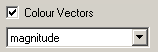
\includegraphics{Ch03/3-9.png}}
\caption{Option to colour the vectors with their magnitude.}
\label{fig:3.14}
\end{figure}

\begin{figure}[H]
\center{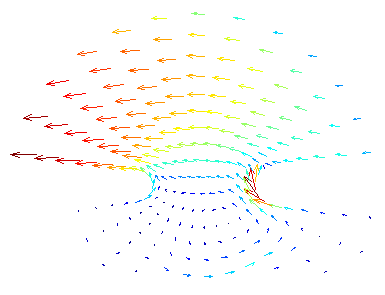
\includegraphics[width=0.5\textwidth]{Ch03/colvectors.png}}
\caption{Vector colour dependent on the velocity magnitude (vector length).}
\label{fig:3.15}
\end{figure}

\section{Data units}
Whenever \QUICKPLOT\ knows the unit of the quantity that you have selected, the data unit conversion option will appear.
The listbox allows you to select the unit system that you want to use for plotting and exporting.
The following options are available: As in file (no conversion carried out), SI (base units: m, kg, s), CGS (base units: cm, g, s), FPS (base units: ft, lb, s), IPS (base units: in, lb, s), NMM (base units: mm, g, s), Other (user specified unit consistent with the original unit), and finally Hide (no units shown in plot).
On start \QUICKPLOT\ reads the unit definitions from the units.ini file stored in the executable directory.
That file contains both long and short names, all names will be recognized as well as combinations with prefixes such as kilo (or k) and milli (or m).
\Fref{fig:DataUnitsManual} shows the Data unit option in the mode in which you can specify your own unit from simple units such as yd or km (as shown) or more complex equivalents thereof such as in$^3$/yd$^2$, i.e. cubic inch per square yard (typed as {in\^{}3/yd\^{}2}).

\begin{figure}[H]
\center{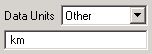
\includegraphics{Ch03/data_units_manual.png}}
\caption{Data unit set to user specified unit.}
\label{fig:DataUnitsManual}
\end{figure}

\section{Angle conventions}
If the vector component selected is an angle then you can select one of the following angle conventions: Nautical To [-180 to 180], Nautical To [0 to 360], Nautical From [-180 to 180], Nautical From [0 to 360], Cartesian To [-180 to 180], Cartesian To [0 to 360], Cartesian From [-180 to 180], Cartesian From [0 to 360].

\section{Vector style}
If the plot type is set such that a vector field is to be plotted (in a horizontal or vertical plane) the vector style can be set.
There are currently three choices: rooted arrow (base of vector located at point at which vector quantity is defined), centred arrow (vector extends in both directions relative to the location at which it is defined), rooted line (combination of point and line, i.e. no arrow head).
\Fref{fig:3.7} shows all three vector styles in action.

\begin{figure}[H]
\center
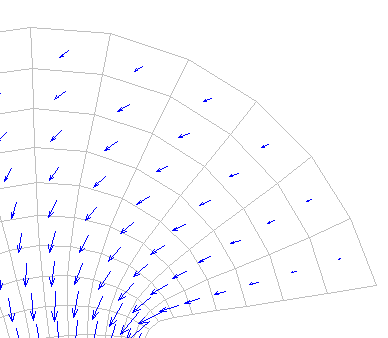
\includegraphics[width=0.3\textwidth]{Ch03/rooted_arrow.png}
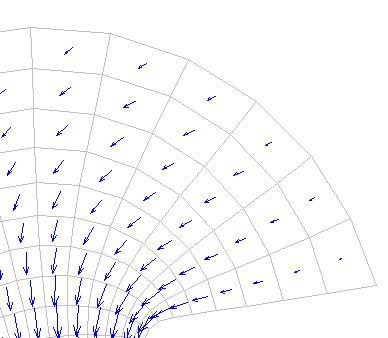
\includegraphics[width=0.3\textwidth]{Ch03/centred_arrow.png}
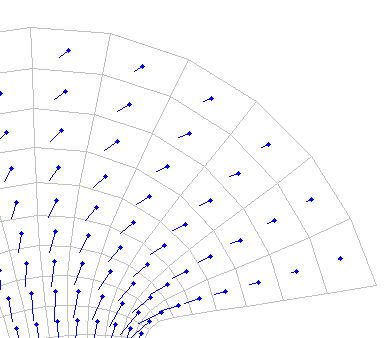
\includegraphics[width=0.3\textwidth]{Ch03/rooted_line.png}
\caption{Example plots of the vector styles.}
\label{fig:3.7}
\end{figure}

\section{Vector scaling} \label{Sec:VectorScaling}
If the plot type is set such that a vector field is to be plotted (in a horizontal or vertical plane) the vector scaling option can be set.
There are four choices: automatic (default), manual, automatic normalised and manual normalised.
If the vector scaling is set to automatic, the vectors in the field are scaled such that the maximum vector length is of the order of the distance between points.
When such a field is animated, the scaling will differ between frames.
If either one of the normalised options is selected all vectors plotted will have the same length (see \Fref{fig:3.9}).

If either one of the options with manual scaling is selected, you are requested to enter a scaling value: a value of 2.5 indicates that a unit vector (e.g.\ 1 m/s) is plotted as a vector of 2.5 m length (see \Fref{fig:VectorScalingManual}).

\begin{figure}[H]
\center{
\includegraphics{Ch03/3-3.png}}
\caption{Vector scaling set to manual.}
\label{fig:VectorScalingManual}
\end{figure}

\begin{Remark}
\item It is not yet possible to get a legend or unit vector in the plot for reference.
\end{Remark}

\begin{figure}[H]
\center{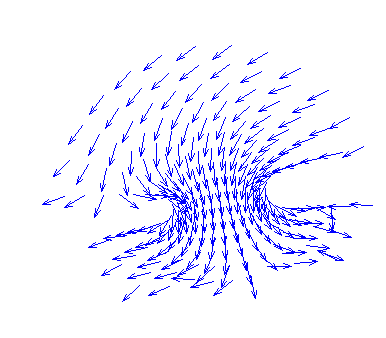
\includegraphics[width=0.5\textwidth]{Ch03/normalised_vector_plot.png}}
\caption{Normalised vector plot (same field as in \Fref{fig:3.4})}
\label{fig:3.9}
\end{figure}

\section{Vertical scaling}
Because most numerical models of natural open waters cover in general a larger domain in the horizontal plane (X, Y distance) than in the vertical plane (Z distance), the vertical scale of a cross-sectional plot is generally exaggerated.
Special care must be taken when plotting vector quantities in such cases.
The default setting of the Vertical Scaling is unrestricted scaling, which means that the vertical scale of the plot automatically adjusts to the vertical space available in the plot; arrows may come out skewed in this case.
If the Vertical Scaling is set to automatic, the vertical scaling is adjusted such that the maximum vertical dimensions are 1/10 of the maximum horizontal dimensions.
If it is set to manual, you can fix the vertical scale relatively to the horizontal scale by setting the enlargement factor.
An enlargement factor of 1 implies an undistorted scale, a factor of 30 indicates a thirty times exaggerated vertical scale.

\begin{figure}[H]
\center{
\includegraphics{Ch03/3-5.png}}
\caption{Vertical scaling set equal to horizontal scaling.}
\label{fig:3.10}
\end{figure}

\begin{figure}[H]
\center{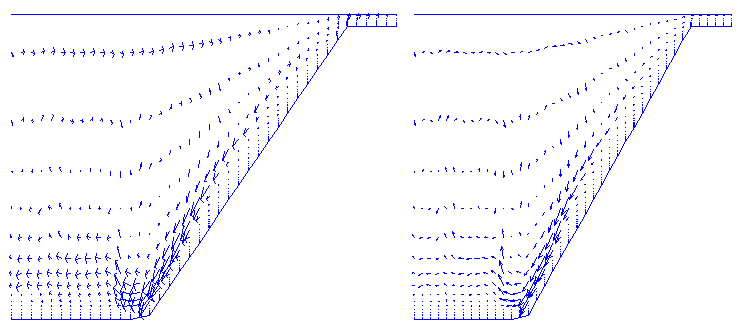
\includegraphics[width=\textwidth]{Ch03/vscale-example.png}}
\caption{Unrestricted vertical scaling on the left (skewed arrows), vertical scaling factor of 100 used on the right (non-skewed arrows: arrows corrected for vertical scaling).}
\label{fig:3.11}
\end{figure}

\section{Formatting of texts}
If the presentation type is set to values, you can specify the size of the font used for displaying the values and the format of the values.
The unit of the font size (default 6) is points.
This is the normal font unit used in most word processors.
The size of the font does not scale with the size of the plot: a cluttered plot on the screen may come out fine on paper.
The main part of the format string for the values is a C-style value format indicator.
This can be \%.df for a floating point value with d decimals behind the decimal point, \%.de for an exponential notation with d+1 decimal places, or \%g for an automatic selection of the display format per value.
Optionally, you can add some text to each value, e.g.\ `depth = \%.2f' although this often increases the cluttering.
Furthermore, the alignment of the values can be set to left, centre, or right (horizontal) and top, cap, middle, baseline, or bottom (vertical).
Non-central alignment is useful when combining different quantities in one plot or when combining markers and values in one plot.

\begin{figure}[H]
\center{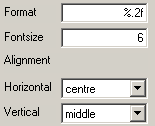
\includegraphics{Ch03/3-8.png}}
\caption{Options available for the formatting of the numerical values.}
\label{fig:3.13}
\end{figure}

\section{Colouring dams}
There are some cases in which thin dams have certain properties (e.g.\ weir heights).
In such cases, you can check the Colour Dams checkbox to colour them based on that value.

\begin{figure}[H]
\center{
\includegraphics{Ch03/3-11.png}}
\caption{Checkbox to indicate optional colouring of thin dam like structures such as weirs.}
\label{fig:3.16}
\end{figure}

\section{Value operator}
For data on edges, which may often include fluxes across the edges, you may select to either plot the actual value (operator: none) or the absolute value (operator: abs).

\section{Colours}
You can change the colour used for line graphs, vector fields, values and uniformly coloured contour lines by clicking on the coloured rectangle of the colour option and selecting the colour from the standard colour interface.
This colour option sets also the colour of the lines if the presentation type is set to patches with lines or contour patches with lines.

\begin{figure}[H]
\center{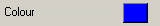
\includegraphics{Ch03/3-13.png}}
\caption{Default colour setting.}
\label{fig:3.18}
\end{figure}

\section{Fill polygons}
If the data contains line data (for instance a land boundary file) you can select the option to Fill Polygons.
When this option is activated, you can set the colour separately.

\begin{figure}[H]
\center{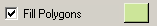
\includegraphics{Ch03/3-14.png}}
\caption{Default colour setting for filled polygons.}
\label{fig:3.19}
\end{figure}

\section{Text box}
When plotting text labels (for instance when the presentation type is set to values) you can add a box around each text.
When this option is activated, you can set the fill colour of the box separately.
The boundary of the box will have the same colour as the text.

\begin{figure}[H]
\center{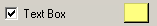
\includegraphics{Ch03/3-15.png}}
\caption{Default colour setting for text boxes.}
\label{fig:3.20}
\end{figure}

\section{Line style} \label{Sec:LineStyle}
In case of a line plot, you can make selection of four line styles: - (continuous line, default), -- (dashed line), : (dotted line) and -. (dash dotted line) combined with an optional marker or switch off the line completely and use a marker only (for marker settings, see \Sref{Sec:Markers}).
The width of the line can also be changed (see \Sref{Sec:LineWidth}).

\begin{figure}[H]
\center{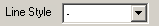
\includegraphics{Ch03/3-16.png}}
\caption{Dropdown list for line style selection.}
\label{fig:3.21}
\end{figure}

\section{Line width} \label{Sec:LineWidth}
Besides the line style you can also set the line width.
The default line width is 0.5 point.

\begin{figure}[H]
\center{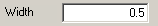
\includegraphics{Ch03/3-17.png}}
\caption{Edit box for the line width.}
\label{fig:3.22}
\end{figure}

\section{Marker settings} \label{Sec:Markers}
If the presentation type is set to marker or if a line plot is created, you have to select the marker type.
There are thirteen markers: + (plus symbol), o (circle), * (star), . (dot), x (times symbol), square, diamond, v (triangle pointing down), $\wedge$ (triangle pointing up), $>$ (triangle pointing right), $<$ (triangle pointing left), pentagram and hexagram.
In case of a line plot, there is the additional option of no marker (none).
By default, the markers are coloured based on the local values in a 2D plot, whereas they are transparent (no filling) and marker colour equals line colour for line graphs.
Optionally, you can set a uniform colour for the marker edge and/or filling.
The markers +, *, . and x do not have a filled area, so you can set only their (edge) colour.

\begin{figure}[H]
\center{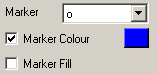
\includegraphics{Ch03/3-18.png}}
\caption{Marker option selecting circles with a blue border and fill colour dependent on the local value.}
\label{fig:3.23}
\end{figure}

\section{Classify colours}
When plotting the data as coloured vectors, patches, patches with lines, and markers, you may choose either to use a continuous colour scale, or a discrete number of colour classes.
The thresholds used for colour classes

\section{Thresholds for contours/colours} \label{Sec:Thresholds}
If the presentation type is set to any of the contouring options, the program will by default plot 10 contours which are automatically selected uniformly between the minimum and maximum value in the plot (or between the limits set in the edit fields of the colour limit option, see \Sref{Sec:ColourLimits}).
The number of contours can be changed by typing a positive integer number in the edit field below the Thresholds label.
The thresholds can be distributed linearly or logarithmic.
If you want even more control over the thresholds, you can specify them in the Thresholds edit box.
You can use the MATLAB colon-notation (minimum : step : maximum or minimum : maximum which uses the default step 1) as a shorthand notation for multiple linearly spaced contour levels, e.g.\ 0:0.5:3 is a shorthand for the list 0 0.5 1 1.5 2 2.5 3.

\begin{figure}[H]
\center{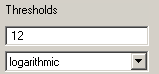
\includegraphics{Ch03/3-12a.png}
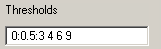
\includegraphics{Ch03/3-12b.png}}
\caption{Contouring threshold options: 12 automatic thresholds logarithmically distributed or 10 user-specified thresholds.}
\label{fig:3.17}
\end{figure}

\begin{Remark}
\item If you want only one contour line at an integer value, say 12, you will have to shift it a little (say, 12.001) to distinguish it from a number indicating the number of automatic contours.
\item Areas below the lowest threshold will be clipped.
Add a big negative value to prevent this.
\end{Remark}

\section{Colour limits} \label{Sec:ColourLimits}
By default the colour limits are determined automatically based on the selected data.
Comparison of results of different simulations and animations require a fixed colour scaling for all plots.
Therefore, an option has been provided to set the colour scaling manually.
In that case change the Colour Limits option from automatic into manual and specify the upper and lower limit of the colour range.
If the colour limits are set automatically, you can force symmetric limits around 0 (i.e., max=+x and min=-x) by checking the Symmetric Limits option.

\begin{figure}[H]
\center{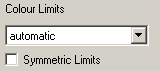
\includegraphics{Ch03/3-19a.png}
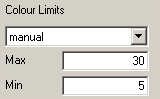
\includegraphics{Ch03/3-19b.png}}
\caption{The colour limits have been set manually to 5 and 30, respectively.}
\label{fig:3.24}
\end{figure}

\begin{Remark}
\item The colour limits influence the automatic selection of contouring thresholds (see \Sref{Sec:Thresholds}).
\end{Remark}

\section{Colour map}
There are currently 25 colour maps to choose from: autumn, avs, bluemap, bone, cool, copper, depth, earth1, earth2, earthsurface, flag, gray, hot, hsv, jet, jet (5\% white band), pastel, pink, qncmap, reversed bluemap, sedconc, spring, summer, winter, xhsv.
All colour maps are shown in \Fref{fig:3.25} from left to right.
The colour map must be selected from the dropdown list below the colour map label.
The colour maps are stored in ASCII files in a subdirectory `colormaps'.
Additional colour maps can be defined and added interactively; how to do this is explained in Section 5.7.

\begin{figure}[H]
\center{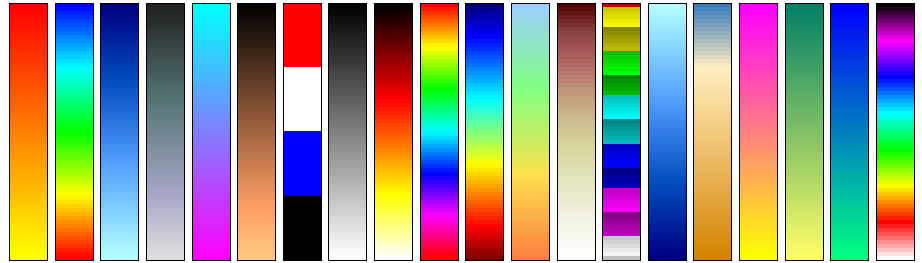
\includegraphics[width=\textwidth]{Ch03/3-20.png}}
\caption{List of colour maps available to the \QUICKPLOT\ user.}
\label{fig:3.25}
\end{figure}

\begin{figure}[H]
\center{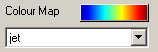
\includegraphics{Ch03/3-21.png}}
\caption{A colour map can be selected from the dropdown list.
The colour map preview will update when another colour map has been selected.}
\label{fig:3.26}
\end{figure}

\section{Colour bar}
If the plot uses a colour map for colouring the data, the colour map can be drawn as a legend to the right (default) or below the plot.
You can set this by checking the concerning checkboxes.

\begin{figure}[H]
\center{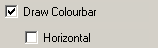
\includegraphics{Ch03/3-22.png}}
\caption{Checkboxes for plotting a vertical (or optionally horizontal) colour bar.}
\label{fig:3.27}
\end{figure}

\section{Field thinning}
A vector field, a field of values or markers can become cluttered when a lot of items are plotted.
Therefore, it is possible to selectively remove some of these items (vectors, values or markers).
Depending on the exact plot options there may be four settings:
\begin{itemize}
\item \emph{none}: No thinning will be applied.
\item \emph{uniform}: This option selects the indices $1$, $p+1$, $2p+1$, ... for each of the M, N and K directions included in the dataset where $p$ is the thinning factor.
\item \emph{distance}: Plot locations are selected that are at least a distance $d$ apart.
\item \emph{dynamic}: This option is only available when plotting labels.
If there are less than $n$ locations in the zoomed area, then all locations are plotted.
If there are more than $n$ locations within the zoomed area, then a subset of $n$ locations is plotted.
If the values are scalar numeric, then the values selected include the smallest and largest values (independent of their separation), otherwise the selection starts with the first data point.
Subsequent locations are selected such that each additional location is the location furthest away from all previously selected locations.
If the initial data set contains more than 50,000 points then a random subset of 50,000 points is used as the first thinning step.
\end{itemize}

\begin{figure}[H]
\center{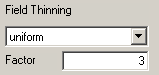
\includegraphics{Ch03/3-23a.png}
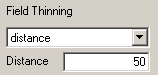
\includegraphics{Ch03/3-23b.png}}
\caption{Optional field thinning based on grid numbers (uniform thinning) or distance.}
\label{fig:3.28}
\end{figure}

\begin{figure}[H]
\center{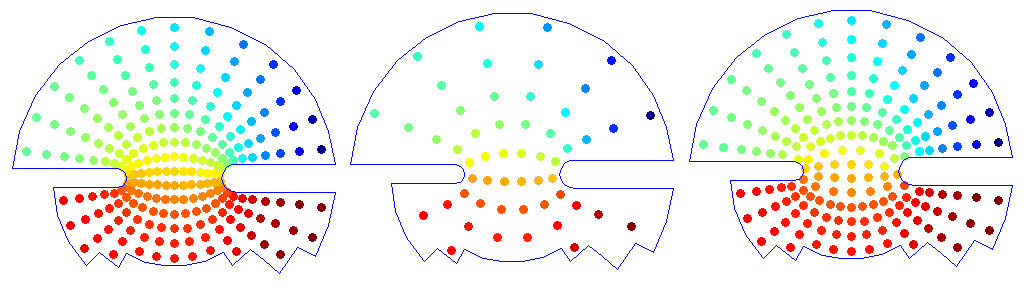
\includegraphics[width=\textwidth]{Ch03/thinning-example.png}}
\caption{Example of a marker plot without thinning (left), uniform thinning (factor 2) and distance thinning (right).}
\label{fig:3.29}
\end{figure}

\section{Clipping data values} \label{Sec:DataClipping}
One of the most powerful plotting options is the clipping functionality.
It allows you to clip/remove certain values from the plot. Default it clips data points equal to -999, but you can clip almost any value or range that you can think of.
Examples:

\begin{itemize}
\item $<0$ Clip all values less than 0.
\item $<=0$ Clip all values less than or equal to 0.
\item $[0\ 4]$ Clip all values larger than or equal to 0 and smaller than or equal to 4.
\item $(0\ 4)$ Clip all values larger than 0 and smaller than 4.
\end{itemize}

Furthermore, it allows you to have any combination of such ranges as shown in \Fref{fig:3.30}.

\begin{figure}[H]
\center{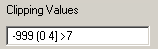
\includegraphics{Ch03/3-25.png}}
\caption{This setting will clip the values equal to -999, or larger than 0 and less than or equal to 4, or larger than 7.}
\label{fig:3.30}
\end{figure}

\begin{Remark}
\item If you clip values in a certain range, for instance between 0 and 4, and two neighbouring data points have values at either side outside the range, say -1 and 5, then a continuous shades plot may still contain some interpolated values in the clipped range.
\end{Remark}

\section{Clipping coordinate values}
Besides clipping data based on the values, it may be useful to clip the data based on $x$ and $y$ coordinates. This is in particular useful if the coordinate data contains dummy values that have not automatically been detected and removed. Although this feature can also be used to clip the plotted domain to a certain $x$,$y$ region, it should be mentioned here that it is more memory efficient to use the $M$,$N$ index space for such clipping.